\documentclass{article}
\usepackage[backend=biber, style=authoryear, sorting=nyt, style=numeric]{biblatex}
\usepackage{url}
\usepackage[dvipsnames]{xcolor}
\usepackage{enumitem}

\usepackage{background}
\usepackage{tikz}
\usepackage{geometry}
\usetikzlibrary{shapes, arrows, positioning}
\usepackage[T1]{fontenc}
\usepackage[utf8]{inputenc}
\usepackage[british]{babel}
\usepackage{titletoc}
\usepackage{titlesec}
\usepackage{lipsum}
\usepackage{tocloft}
\usepackage{hyperref}
\usepackage{algorithm}
\usepackage{algpseudocode}
\usepackage{graphicx}
\usepackage[section]{placeins}
\usepackage{caption}
\usepackage{textcomp}
\usepackage{subcaption}
\usepackage[edges]{forest}
%\usepackage[superscript,biblabel]{cite}
\usepackage{fontawesome5}
\usepackage{algorithm}
\usepackage{algpseudocode}
\usepackage{amsmath}
\usepackage[simplified]{pgf-umlcd}
\usepackage{enumitem}
\usepackage{adjustbox}
\usepackage{listings}
\usetikzlibrary{shapes.geometric, arrows}
%\usepackage[style=ext-authoryear, backend=biber]{biblatex}
%\usepackage{url}
%\usepackage[style=authoryear]{biblatex}
\addbibresource{rapport.bib}
%\usepackage{cite}
\usepackage[british]{datetime2} % Enhanced date and time.

\addbibresource{rapport.bib}

\definecolor{aerospaceblue}{RGB}{0, 128, 255} % Couleur bleu ciel pour l'aérospatiale
\definecolor{myblue}{RGB}{0, 0, 255}

% Define the theme colors
\definecolor{blue}{RGB}{0,0,255}
\definecolor{green}{RGB}{0,128,0}
\definecolor{red}{RGB}{255,0,0}
\definecolor{custompurple}{RGB}{128,0,128}

% Set the lstset configuration
\lstset{
	language=C++,
	basicstyle=\ttfamily\small,
	keywordstyle=[1]\color{blue},
	keywordstyle=[2]\color{black},
	keywordstyle=[3]\color{green!60!black},
	commentstyle=\color{green!60!black},
	stringstyle=\color{red},
	otherkeywords={CALL},
	morekeywords=[1]{CALL},
	morekeywords=[2]{FOPENSUBNODES},
	numbers=left,
	numberstyle=\tiny,
	stepnumber=1,
	numbersep=5pt,
	frame=single,
	breaklines=true,
	breakatwhitespace=true,
	tabsize=4,
	captionpos=b,
	showstringspaces=false,
	% Adjust the frame margins for a larger rectangle
	xleftmargin=1em,
	framexleftmargin=1em,
	framexrightmargin=1em
}


\tikzset{
	startstop/.style={
		rectangle,
		rounded corners,
		minimum width=3cm,
		minimum height=1cm,
		text centered,
		draw=black,
		fill=red!30
	},
	io/.style={
		trapezium,
		trapezium stretches=true, % A later addition
		trapezium left angle=70,
		trapezium right angle=110,
		minimum width=3cm,
		minimum height=1cm,
		text centered,
		draw=black,
		fill=blue!30
	},
	process/.style={
		rectangle,
		minimum width=3cm,
		minimum height=1cm,
		text centered,
		text width=3cm,
		draw=black,
		fill=orange!30
	},
	decision/.style={
		diamond,
		minimum width=3cm,
		minimum height=1cm,
		text centered,
		draw=black,
		fill=green!30
	},
	arrow/.style={
		thick,
		->,
		>=stealth
	}
}

\newcommand{\coloredsquare}[1]{\textcolor{#1}{\rule{1em}{1em}}}

\renewcommand{\cfttoctitlefont}{\hfill\large\bfseries\fontsize{20}{24}\selectfont}
\renewcommand{\cftaftertoctitle}{\hfill\mbox{}}

\definecolor{mydarkyellow}{HTML}{87CEEB}
\definecolor{lightblue}{RGB}{173,216,230}
\definecolor{lightyellow}{RGB}{255,255,204}
\definecolor{yellow}{RGB}{255,255,0}

\backgroundsetup{
	scale=1,
	color=black,
	opacity=0.5,
	angle=0,
	contents={
		\ifnum\value{page}=1
		\begin{tikzpicture}[remember picture,overlay]
			\path [fill=mydarkyellow] (current page.south west) rectangle (current page.north east);
		\end{tikzpicture}
		\fi
	}
}

\title{\textbf{\Huge Project Report}\\[1cm]
	\textbf{\LARGE Polytech Nice}\\[2cm]
	\hrule height 1pt
	\vspace{0.5cm}
	\textbf{\Large Simple Road Traffic Modeling}\\[0.5cm]
	\hrule height 1pt
	\vspace{3cm}
	\small{\today{}}}

\author{
	\begin{tabular}{c}
		Gerbaud Florent \\ Fatima Rharrour \\ \\
		9-th october to 20-th December september 2023\\
		\\ Academic tutor : Didier Auroux
	\end{tabular}
}

\date{}
\begin{document}
	\maketitle
	\hspace{2cm}
	\begin{figure}[b]
		\centering
		\begin{minipage}[b]{0.45\linewidth}
			
\includegraphics[width=5cm]{logo.png} \\
			%Company tutor : Vincent Vadez
		\end{minipage}
		\hfill
		\begin{minipage}[b]{0.45\linewidth}
			\raggedleft
			\vspace{-0.5cm}
			
\includegraphics[width=6cm]{Polytech.png} \\
			%Academic tutor : Cédric Boulbe
		\end{minipage}
	\end{figure}
	\newpage % ajout d'un saut de page
	% Table des matières
	\renewcommand{\contentsname}{
		\hfill
		
\begin{tikzpicture}
			\node[draw, fill=white, inner sep=20pt,line width=1.5pt] {\fontsize{30}{36}\selectfont\bfseries Table of Contents};
		\end{tikzpicture}
		\hfill
	}
	\tableofcontents
	\newpage
	\listoffigures % Add a listing of figures
	
	\listofalgorithms
	\newpage
	\section{Presentation of the Subject}
	\subsection{Useful Definition}
		\textbf{\underline{Ordinary Differential Equation (ODE):}} \newline\newline
		An ODE is a mathematical equation that relates a function to its derivatives with respect to one or more independent variables. ODEs are commonly represented given a function F of x, y, and derivatives of y. Then, an equation of the form
		\begin{align*}
			F\left(x,y,y',\ldots ,y^{(n-1)}\right)=y^{(n)}
		\end{align*}
		
		\textbf{\underline{What is Road Traffic Modeling}} \newline\newline
		The Road Traffic modeling  is the study of how vehicles behave on road networks, aiming to simulate and analyze various aspects of traffic flow, congestion, and driver behavior. This field involves creating mathematical and computer models to understand and predict traffic patterns, particularly in scenarios such as congestion, erratic driving, and other relevant factors affecting road transportation. Road traffic modeling plays a crucial role in urban planning, traffic management, and the development of intelligent transportation systems (you could see an exemple on the \ref{fig:intro}).
	
	\subsection{Simple Road Traffic Modeling}
	
		Here explain what is the objective how we are going to do the study and so on \cite{JEIHANI2017164}
		
		\begin{figure}[H]
			\centering
			\includegraphics[width=0.8\textwidth]{intro.jpg}
			\caption{\textbf{\underline{Road traffic : }} In this picture, you can see an example of a road traffic phenomenon that we could study}
			\label{fig:intro}
		\end{figure}
	
		
		\subsubsection{The objective of SMRT}
		The primary objective of simple road simulation is to analyze and understand the behavior of vehicles in a controlled and reproducible environment. By simulating basic road conditions, researchers and engineers can study the impact of various factors on traffic flow, safety, and efficiency. This helps in the development and testing of traffic management strategies and vehicle control systems. Simple road simulations provide a valuable tool for investigating the dynamic interactions between vehicles and the road environment, contributing to advancements in transportation research and technology.
		
		\subsubsection{Use case to explain the interest of these simulations}
		Simple road simulations find applications in various fields, such as urban planning, transportation engineering, and autonomous vehicle development. For instance, they can be used to assess the effectiveness of new traffic signal timings, study the implications of road design changes, or test the performance of autonomous vehicles in different traffic scenarios. These simulations provide a cost-effective and risk-free way to evaluate potential real-world interventions and innovations. The ability to model and analyze diverse road scenarios enhances decision-making processes and supports the development of sustainable and efficient transportation systems.
		
		\subsubsection{Field of application}
		Simple road simulation is applied across a wide range of fields, including but not limited to transportation research, traffic engineering, and urban planning. Additionally, it plays a crucial role in the development and validation of autonomous vehicle technologies. The ability to model and simulate various road conditions helps researchers and practitioners make informed decisions and improvements in the design and management of transportation systems. Simple road simulation serves as a powerful tool for enhancing our understanding of traffic dynamics and contributes to the ongoing evolution of smart and adaptive transportation systems.
	
	\subsubsection{Using GitHub for Project Management}
	
	\begin{figure}[H]
		\centering
		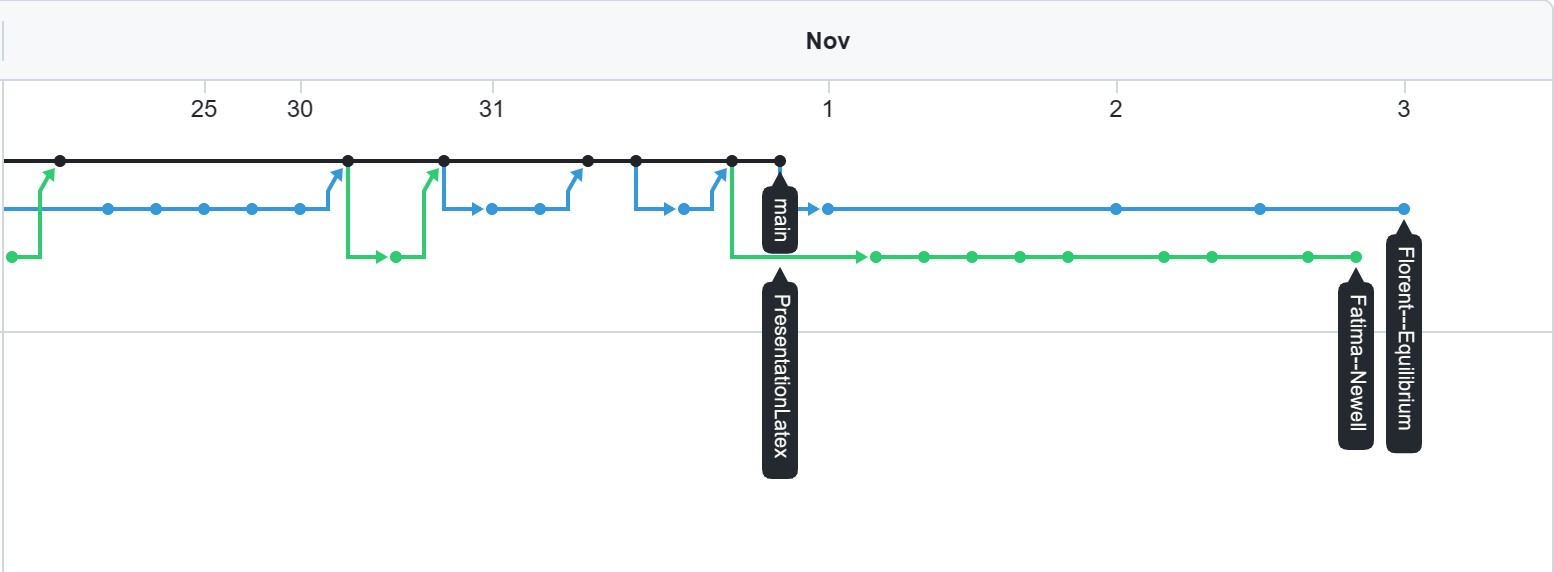
\includegraphics[width=0.8\textwidth]{GitHub.jpg}
		\caption{\textbf{\underline{Road traffic : }} In this picture, you can see an example of a road traffic phenomenon that we could study}
		\label{fig:GitHub}
	\end{figure}
	
	\section{The equation for SMRT}
		\subsection{Differential Ordinary Equation }
		In this part, the idea is to resolve two types of systems of Ordinary Differential Equations (ODEs) that allow us to simulate traffic flow. To achieve this, we will use the Euler Explicit method to numerically solve the solutions.
		The Euler Explicit method is given by the folowing eqution :
		\begin{itemize}
			\item EDO to solve: $\boxed{y'(t) = f{\bigl (}t, y(t){\bigr )}}$.
			\item First step of the resolution: $\boxed{y_0 = y(t_0)}$.
			\item Recursive process to find the n-th solution of the EDO: $\boxed{y_{n+1} = y_{n} + hf(t_{n}, y_{n})}$
		\end{itemize}
		
		
		
		
		
		\subsubsection{Linear Model}
			\textbf{\underline{Mathematical Theory:}}
			\newline
			
			In this section, we're going to explain the math behind our model for understanding how cars behave in traffic. To make things simple, we use a discrete model, which means we look at cars one at a time and how they interact on the road.
			
			Each car's movement is governed by a basic equation:
			
			\begin{align*}
				\dot{x_i}(t) = V_i = \alpha_i(x_{i-1} - x_i)
			\end{align*}
			
			In this equation, \(x_i(t)\) represents where the \(i\)-th car is at a given time, \(V_i\) is how fast the \(i\)-th car is going, and \(\alpha_i\) is a number that describes how that car behaves. The right side of the equation, \(\alpha_i(x_{i-1} - x_i)\), tells us how the car's speed changes based on how close it is to the car in front.
			
			When we put this equation to work for all the cars, we end up with a bunch of equations (one for each car), which helps us understand how they all move together in traffic. These equations give us a dynamic view of how cars influence each other as they drive.
			
			The system of equations is written like this for each car, where \(i\) can be 1, 2, and so on, up to the number of cars:
			
			\begin{align*}
				\left\{
				\begin{array}{ll}
					\dot{x}_1 &= V_1 \\
					\dot{x}_2(t) &= \alpha_2(x_1 - x_2) \\
					&\vdots \\
					\dot{x}_n(t) &= \alpha_n(x_{n-1} - x_n)
				\end{array}
				\right.
			\end{align*}
			
			These equations help us understand how traffic flows and how individual cars influence one another on the road.
			
			In the first part of the study, we consider $\alpha_i$ as a constant. However, in the next part of the simulation, we define some functions $\alpha_i(t)$.
			
			In fact, we have three types of simulations:
			
			1. \textbf{\underline{Constant value:}}
			\[
			\alpha_i(t) = C_i
			\]
			
			2. \textbf{\underline{Sinusoidal with noise:}}
			\[
			\alpha_i(t) = \left| W \cdot \sin(\omega t + \phi) + \mathcal{N}(0, 0.1) \right|
			\]
			
			3. \textbf{\underline{Stochastic Driver Model:}} \newline \newline
			Consider a random driver model with an output labeled as \( \alpha_i(t) \), which relies on various factors like the average, spread, and time \( t \). This model produces a random noise part from a usual distribution with an average and spread of \( \sqrt{\text{spread}} \). If a limit is given, the generated noise is confined within the interval \([- \text{limit}, \text{limit}]\). \newline \newline
			
			\textbf{Mathematically, we can express this as:}
		
			
			\[
			\alpha_i(t) =
			\begin{cases}
				\left| \mathcal{N}(\text{average}, \sqrt{\text{spread}}) \right|, & \text{if } -\text{limit} \leq \alpha_i(t) \leq \text{limit}, \\
				-\text{limit}, & \text{if } \alpha_i(t) < -\text{limit}, \\
				\text{limit}, & \text{if } \alpha_i(t) > \text{limit}.
			\end{cases}
			\]
			
			Here, \( \text{average} \) signifies the mean of the acceleration, and \( \text{spread} \) stands for the acceleration's spread. The limit is defined to prevent or create specific situations, like accidents, depending on the desired result. \\
			
			
			\textbf{\underline{Implementation : }}
			
			\begin{algorithm}[H]
				\caption{$\dot{x_1}$}\label{alg:x1_dot}
				\begin{algorithmic}
					%\State \textbf{Input:} \\
					%\begin{itemize}
						%\State $P_1,P_2,P_3,:=\text{"the 3 first vertex of the 2D mesh"}$
					%\end{itemize}
					\State \textbf{Output:} \\
					\begin{itemize}[]
						\item $\dot{x_1}=V_1$
					\end{itemize}
					\State \textbf{Algorithm:} \\
					\begin{itemize}[]
						\State $\dot{x_1}=130 \times \frac{1000}{3600}$ 
						\State \Return $\dot{x_1}$ 
					\end{itemize}		
				\end{algorithmic}
			\end{algorithm}
			
			\begin{algorithm}[H]
				\caption{$\dot{x_i}$}\label{alg:xi_dot}
				\begin{algorithmic}
					\State \textbf{Input:} \\
					\begin{itemize}
					\State $t:=\text{"time  step"}$
					\State$x_i:=\text{Table of position for the i-th Car}$
					\State$x_{i-1}:=\text{Table of position for the (i-1)-th Car}$
					\end{itemize}
					\State \textbf{Output:} \\
					\begin{itemize}[]
						\item $\dot{x_i}=V_i$
					\end{itemize}
					\State \textbf{Algorithm:} \\
					\begin{itemize}[]
						\State $\dot{x_i}(t) = V_i = \alpha_i(x_{i-1}[t] - x_i[t])$ 
						\State \Return $\dot{x_i}$ 
					\end{itemize}		
				\end{algorithmic}
			\end{algorithm}
			
			This algorithm allows to define an orthonormed local reference frame and we delete the lines to eliminate for reducing matrix
			
			\begin{algorithm}[H]
				\caption{sinusoidal\_model}\label{alg:sinusoidal_model}
				\begin{algorithmic}
					\State \textbf{Input:} \\
					\begin{itemize}
						\State $W := \text{"Amplitude of the perturbation"}$
						\State $\omega := \text{"Angular frequency"}$
						\State $t := \text{"time"}$
						\State $\phi := \text{"Phase (in radians)"}$
					\end{itemize}
					\State \textbf{Output:} \\
					\begin{itemize}
						\item This function returns a value of acceleration $(\alpha_i(t))$ following a sinusoidal model with random noise.
					\end{itemize}
					
					\State \textbf{Algorithm:} \\
					\begin{itemize}
						\State $ \alpha_i(t) = \left| W \cdot \sin(\omega \cdot t + \phi) + N \right|$ 
						\State \text{$N$:="random noise such as N $\sim$ $\mathcal{N}(0,0.01)$"}
						\State \Return $\alpha_i(t)$
					\end{itemize}
				\end{algorithmic}
			\end{algorithm}
			
			\begin{algorithm}[H]
				\caption{Update Positions and Velocities}\label{alg:update_positions}
				\begin{algorithmic}
					\State \textbf{Input:} \\
					\begin{itemize}
						\State $t:=\text{time step}$
						\State $x_1Pos:=\text{Table of position for the 1st Car}$
						\State $x_2Pos:=\text{Table of position for the 2nd Car}$
						\State $v_1:=\text{Table of velocity for the 1st Car}$
						\State $v_2:=\text{Table of velocity for the 2nd Car}$
						\State $time:=\text{Table of time values}$
						\State $h:=\text{time step size}$
					\end{itemize}
					\State \textbf{Output:} \\
					\begin{itemize}
						\item $x_1Pos$ \\
						\item $x_2Pos$
					\end{itemize}
					\begin{itemize}[]
						\item $accident:=\text{Flag indicating whether an accident occurred}$
					\end{itemize}
					\State \textbf{Algorithm:} \\
					\begin{itemize}[]
						\For{$t$ in range(1, $n\_steps$)}
						\State $x_1Pos[t] = x_1Pos[t-1] + \dot{x_1}() \times h$
						\State $x_2Pos[t] = x_2Pos[t-1] + \dot{x_2}(t-1) \times h$
						
						\State $v_1[t] = \dot{x_1}()$
						\State $v_2[t] = \dot{x_2}(t)$
						
						\State $time[t] = time[t-1] + h$
						
						\If{isAccident($t$)}
						\State $accident = \text{True}$
						\State \textbf{break}
						\EndIf
						\EndFor
					\end{itemize}
					\State \textbf{Return} $x_1Pos$, $x_2Pos$
				\end{algorithmic}
			\end{algorithm}
			
			
			
		\subsubsection{Newell's Model}
		\subsection{Partial Differential Equations}
		
	\section{Project Objectives}
	\subsection{Problems Encountered}
	
	\section{Types of Simulations Performed}
		\subsection{Simulation with Drunk Drivers}
		\subsection{Simulation with Unpredictable Drivers}
		\subsection{Simulation with Drivers Reacting Similarly}
		\subsubsection{Accordion Phenomenon}
		
		The initial simulation we aimed to conduct was intended to demonstrate and illustrate the behavior of drivers in real-life scenarios. Figure \ref{fig:Aco1} accurately depicts this phenomenon. Specifically, we make the following assumptions:
		
		\begin{itemize}
			\item The first car maintains a constant speed over time.
			\item The second car reaction is based on the behavior of the first one.
			\item The acceleration of the second car is governed by a constant function, denoted as alpha, which remains fixed. In the algorithm \ref{alg:xi_dot} we took $\alpha_2=2.0$
		\end{itemize}
		
		Similar to real-life situations, we observe that if the second car is too far behind the first one, it decelerates. Conversely, when it is adequately distant from the first car, it increases its speed.
		
			\begin{figure}[H]
				\centering
				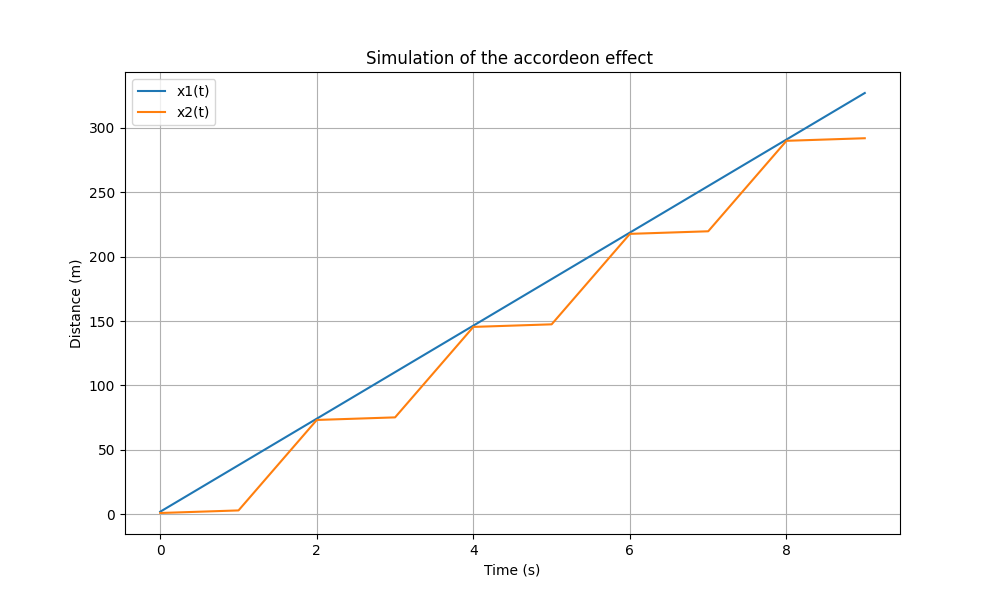
\includegraphics[width=0.8\textwidth]{Accordeon1.png}
				\caption[Simulation of accordion phenomenon]{\textbf{\underline{Simulation of accordion phenomenon : }} In this picture, you can observe the position evolutions of two cars, the first one (blue) maintaining a constant speed, and the second one (orange) following behind the first one. We could see that orange graph behaves like a periodic accordion with respect to time.}
				\label{fig:Aco1}
			\end{figure}
			
			
		\subsubsection{Accident Phenomenon}
		
		For this case, the objectif is to show that if one driver have a bigger time reaction capacity, there is an accident.
		Onto this case, we took the same assumptions than before, but with a capacity of accelleration a little bit lower and a highter time reaction. In the algorithm \ref{alg:xi_dot} we took $\alpha_2=1.75$ and in the algorithm \ref{alg:update_positions} we took $h=1.5$
		
		On the figure \ref{fig:Acc1} accident is confirmed because there is a curve intersection (the position of the car number two (orange) is greater than the first car (blue)) So it means that the second car is crashed into the first car.
		
		\begin{figure}[H]
			\centering
			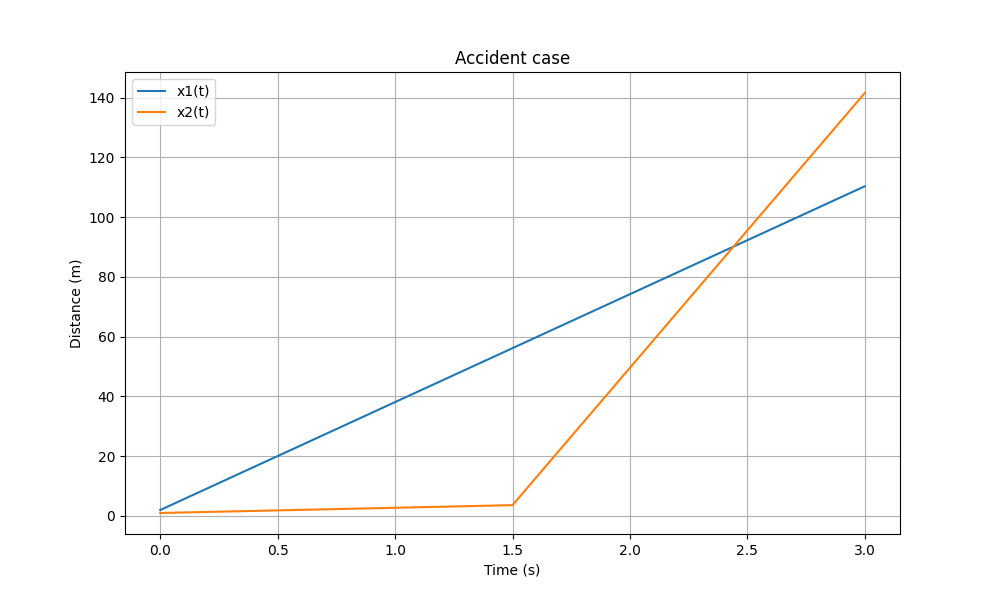
\includegraphics[width=0.8\textwidth]{Acc1.png}
			\caption[Simulation of Accident case between two cars]{\textbf{\underline{Simulation of Accident case between two cars : }} In this picture, you can observe the position evolutions of two cars, the first one (blue) maintaining a constant speed, and the second one (orange) following behind the first one. We could see on The graph shows that the acceleration of the orange car is too large. This implies an accident between two cars.}
			\label{fig:Acc1}
		\end{figure}
		
		\subsection{Study of Equilibrium, Stability, and Instability of the Solution}
		\subsubsection{System Stability and Equilibrium for the Linear Model}
		In this part, the idea is to study the distance difference between two cars in order to determine in which case the solutions is stable and if there is an equilibrium for the solution.
		For doing that, we studied the solutions of the following  system of equation : 
		\begin{align*}
			\begin{cases}
				\dot{d_1} &= V_1 - \alpha_2 \cdot d_1 \\
				&\vdots \\
				\dot{d_n} &= \alpha_n \cdot d_{n-1} - \alpha_{n+1} \cdot d_n
			\end{cases}
		\end{align*}
		
		So, In our context, for the two cars, we have a 1D system. With 3 cars, we have a 2D system of equations.
		
		Now talk about the system stability and equilibrium : 
		\newline \newline \textbf{\underline{With 2 cars}} : \newline\newline
	
		So, the equation to study is the following one : 
		
		\begin{align*}
			\dot{d_1} &= V_1 - \alpha_2 \cdot d_1
		\end{align*}
		
		
		After the resolution (\ref{eq:EDO1}) we obtain the next equation for $d_1(t)$ : 
		\begin{align*}
			\boxed{d_1(t) = \frac{{V_1 - V_1 \cdot e^{-\alpha_2(t-t_0)} + \alpha_2 \cdot d_1(t_0) \cdot e^{-\alpha_2(t-t_0)}}}{\alpha_2}}
		\end{align*}
		
		The first intuition before seeing the equation was to think that when the $\alpha_2 < 0 $, the solution is divergent because one car is go back and the other go forward. Now, if we study the Equation,
		
		the terms $V_1$ and $\alpha_2 \cdot d_1(t_0)$ are constant so they are not interesting.
		
		However, it's important to note that both terms, $e^{-\alpha_2(t-t_0)}$, are exponential functions of time. If the value of $\alpha_2$ is negative, these exponentials will increase exponentially over time.
		
		So we could easily see that the equation is stable and converge onto the equilibrium $d_1(t)=\frac{V_1}{\alpha_2}$.
		
		graphically  we can see it by : 
		
		\begin{figure}[H]
			\centering
			\begin{minipage}[t]{0.50\linewidth}
				\centering
				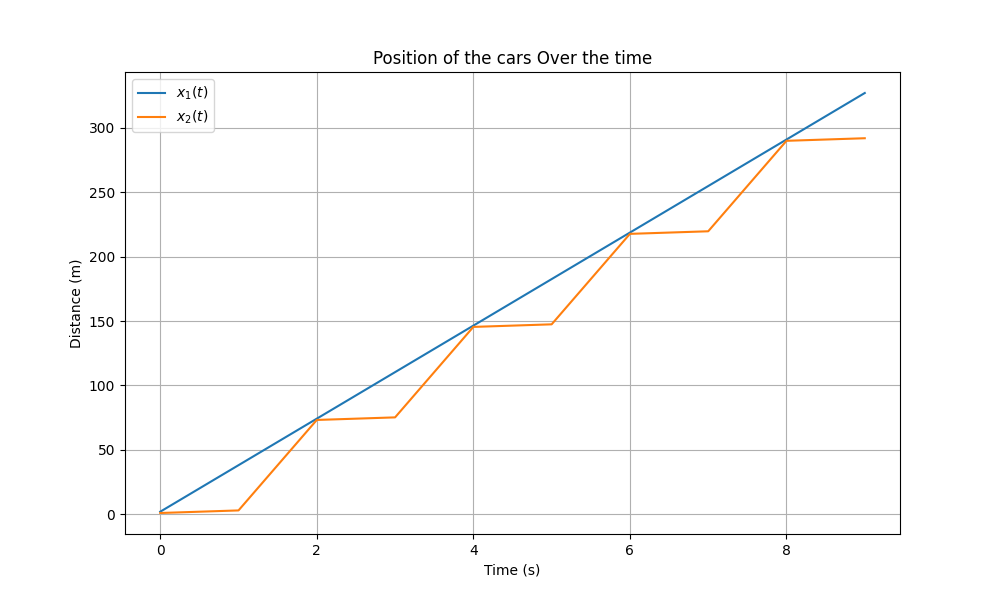
\includegraphics[width=1.4\linewidth]{RealisticCase.png}
				\caption{View of the old window of temrec3D}
				\label{fig:OV}
			\end{minipage}
			\hfill
			\begin{minipage}[t]{0.50\linewidth}
				\centering
				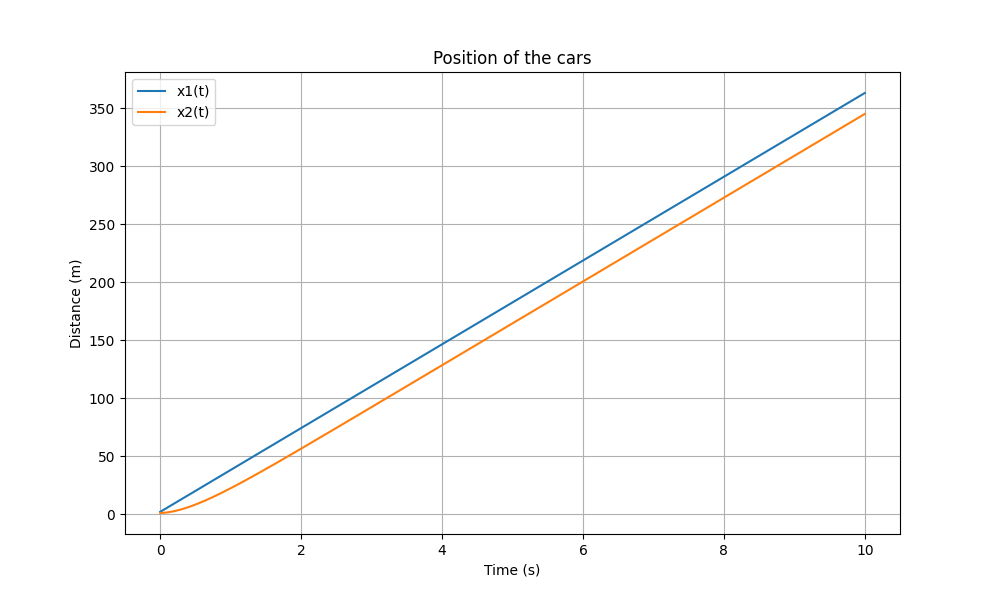
\includegraphics[width=1.4\linewidth]{RealSolCase.png}
				\caption{View of the new window of temrec3D}
				\label{fig:NV}
			\end{minipage}
		\end{figure}
		
		\begin{figure}[H]
			\centering
			\begin{minipage}[t]{0.50\linewidth}
				\centering
				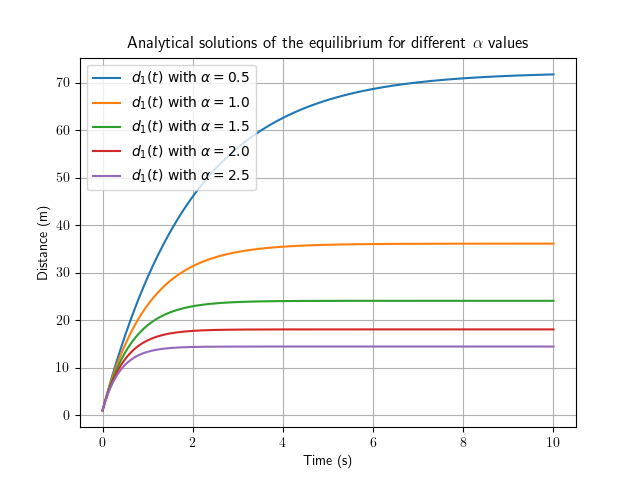
\includegraphics[width=1.4\linewidth]{Stability.png}
				\caption{View of the old window of temrec3D}
				\label{fig:OV}
			\end{minipage}
			\hfill
			\begin{minipage}[t]{0.50\linewidth}
				\centering
				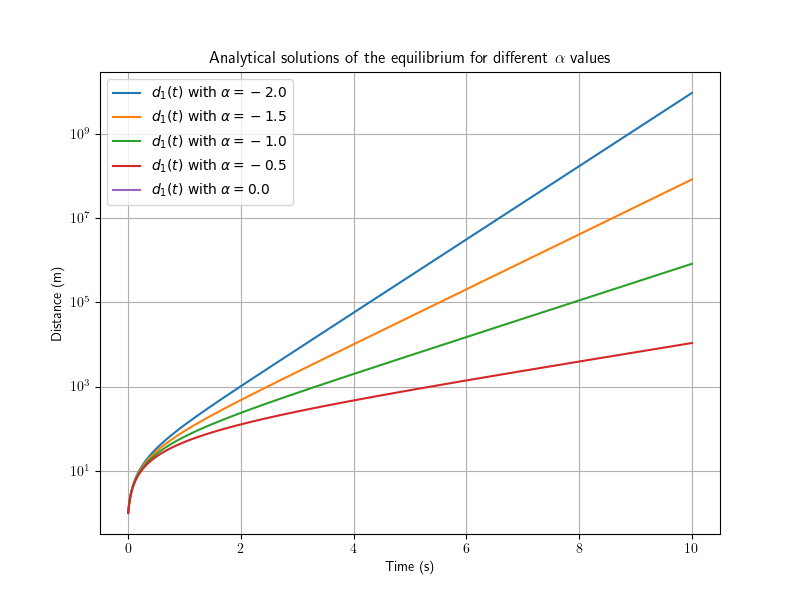
\includegraphics[width=1.4\linewidth]{Unstability.png}
				\caption{View of the new window of temrec3D}
				\label{fig:NV}
			\end{minipage}
		\end{figure}
		
		\begin{figure}[H]
			\centering
			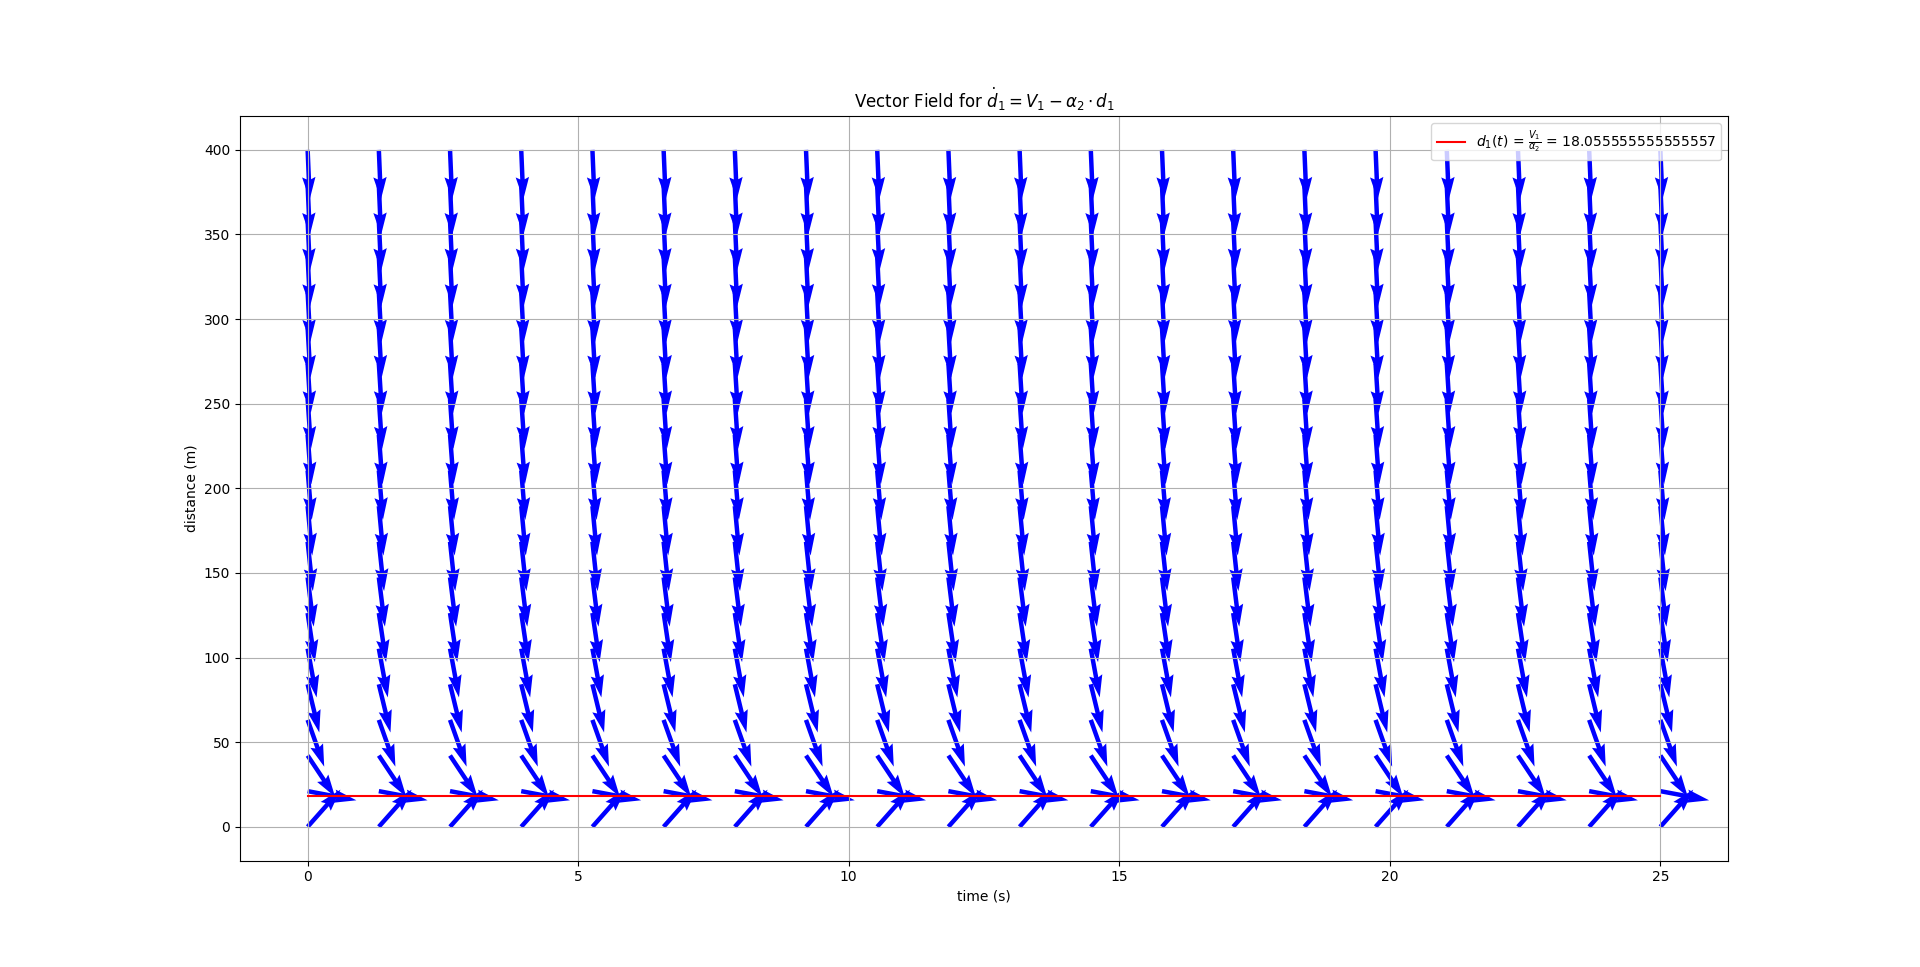
\includegraphics[width=0.8\textwidth]{FieldOfVector_CV.png}
			\caption{\textbf{\underline{Road traffic : }} In this picture, you can see an example of a road traffic phenomenon that we could study}
			\label{fig:GitHub}
		\end{figure}
		
		\textbf{\underline{With 3 cars}} : \newline\newline
		
		After the resolution (\ref{eq:EDO2}) we obtain the next equation for $d_1(t)$ and $d_2(t)$ : 
		
	\subsubsection{System Stability and Equilibrium for the Newell's Model}
	
	\textbf{\underline{The Study of the equilibrium for two cars : }} \newline\newline
	
	
	The objective here, as before, is to study the stability of the model. The 1D equation is as follows:
	
	\begin{align*}
		&\dot{d_1}(t) = \dot{x_1}(t) - \dot{x_2}(t) = V_1 - V_2 + V_2 \cdot e^{-\frac{\alpha_2}{V_2}(d_1 - d_{2}^{sec})} = f(d_1, t), \\
		&\left\{
		\begin{aligned}
			V_1 &:= \text{Maximum speed for car number 1}, \\
			V_2 &:= \text{Maximum speed for car number 2}, \\
			\alpha_2 &:= \text{capacity of acceleration for car number 2}, \\
			d_{2}^{sec} &:= \text{security distance that car number 2 maintains}.
		\end{aligned}
		\right.
	\end{align*}
	
	Firstly, let's determine the equilibrium:
	
	\begin{align*}
		V_1 - V_2 + V_2 \cdot e^{-\frac{\alpha_2}{V_2}(d_1 - d_{2}^{sec})} &= 0 \\
		e^{-\frac{\alpha_2}{V_2}(d_1 - d_{2}^{sec})} &= \frac{V_2-V_1}{V_2} \\
		e^{-\frac{\alpha_2}{V_2}d_1} &= \frac{V_2-V_1}{V_2}e^{-\frac{\alpha_2}{V_2}d_2} \\
		-\frac{\lambda_2}{V_2}d_1 &= \ln \left(\frac{V_2-V_1}{V_2}e^{-\frac{\alpha_2}{V_2}d_2} \right) \\
		d_1^* &= -\frac{V_2}{\lambda_2}\ln \left(\frac{V_2-V_1}{V_2}e^{-\frac{\alpha_2}{V_2}d_2} \right)
	\end{align*}
	
	The challenge with this equation is the inability to find an analytical solution. Consequently, we apply Lyapunov's Indirect Theorem to investigate the equilibrium.
	
	In the context of 1D analysis, we begin by calculating $f'(d_1, t)$, which results in:
	
	\[
	f'(d_1, t) = -\alpha_2e^{-\frac{\alpha_2}{V_2}(d_1 - d_{2}^{sec})}
	\]
	
	It is evident that $f'(d_1, t)$ is negative for all values of $\alpha_2$ greater than zero. Therefore, in our specific scenario, the equilibrium remains stable at all times, as negative acceleration is not considered.
	
	From the equilibrium, we also observe that the equilibrium exists if and only if $V_2 > V_1$.
	
	Clearly, the condition for a stable equilibrium is $\alpha_2 > 0$ and $V_2 > V_1$.
	
	
	\textbf{\underline{The Study of the equilibrium for three cars : }} \newline\newline
	
	\begin{align*}
		&\begin{cases}
			\begin{aligned}
				&\dot{d_1}(t) = \dot{x_1}(t) - \dot{x_2}(t) = V_1 - V_2 + V_2 \cdot e^{-\frac{\alpha_2}{V_2}(d_1 - d_{2}^{sec})} = f(d_1, t), \\
				&\dot{d_2}(t) = \dot{x_2}(t)-\dot{x_3}(t) = V_2 - V_2 \cdot e^{-\frac{\alpha_2}{V_2}(d_1 - d_{2}^{sec})} - V_3 + V_3 \cdot e^{-\frac{\alpha_3}{V_3}(d_2 - d_{3}^{sec})}
			\end{aligned}
		\end{cases}
		 \\
		&\left\{
		\begin{aligned}
			V_1 &:= \text{Maximum speed for car number 1}, \\
			V_2 &:= \text{Maximum speed for car number 2}, \\
			\alpha_2 &:= \text{capacity of acceleration for car number 2}, \\
			d_{2}^{sec} &:= \text{security distance that car number 2 maintains}.
		\end{aligned}
		\right.
	\end{align*}
	
	again, we apply Lyapunov's Indirect Theorem to investigate the equilibrium.
	
	
	We are going to calculkate the Jacobienne matrix : 
	
	\begin{align*}
		J_{\bar{x}}=\begin{pmatrix}
			-\alpha_2e^{-\frac{\alpha_2}{V_2}(d_1 - d_{2}^{sec})} & 0 & \\
			\alpha_2e^{-\frac{\alpha_2}{V_2}(d_1 - d_{2}^{sec})} & -\alpha_3e^{-\frac{\alpha_3}{V_3}(d_2 - d_{3}^{sec})} &
		\end{pmatrix}
	\end{align*}
	
	However, in the 2D case, Lyapunov tells us that the equilibrium is stable if:
	
	\[
	\boxed{
		\begin{aligned}
			Tr(J_{\bar{x}}) &< 0 \\
			\det(J_{\bar{x}}) &> 0
		\end{aligned}
	}
	\]

	The both condition are respected iff $\lambda_2>0, \lambda_3>0$
	\section{Summary}
	
	\section{Annexe}
	
	\subsection{Calculation of the Analytical solutions}
	
	\subsubsection{Linear Model for Two Cars}
	
	\label{eq:EDO1}
	\begin{align*} 
		\dot{d_1}(t) = V_1 - \alpha_2 \cdot d_1
	\end{align*}
	We use the variable separation method to Solve this EDO, so we obtain : 
	\begin{align*} 
		&\int_{x(t_0)}^{x(t_f)} \frac{1}{V_1 - \alpha_2 \cdot d_1(t)} d \ d_1(t) = \int_{t_0}^{t_f} dt \\
		&-\frac{1}{\lambda_2} \left[ \ln\left| V_1 - \alpha_2 \cdot d_1(t) \right| \right]_{x(t_0)}^{x(t_f)} = t_f-t_0 \\
		&-\frac{1}{\lambda_2} \ln\left| \frac{V_1 - \alpha_2 \cdot d_1(t_f)}{V_1 - \alpha_2 \cdot d_1(t_0)} \right| = t_f-t_0
	\end{align*}
	We could remove the |.| because the sign is always the same. And we get : 
	
	\begin{align*}
		&\ln\left( \frac{V_1 - \alpha_2 \cdot d_1(t_f)}{V_1 - \alpha_2 \cdot d_1(t_0)} \right)  = -\lambda_2( t_f-t_0)\\
		&\frac{V_1 - \alpha_2 \cdot d_1(t_f)}{V_1 - \alpha_2 \cdot d_1(t_0)}  = e^{-\lambda_2( t_f-t_0)} \\
		&V_1 - \alpha_2 \cdot d_1(t_f)   = (V_1 - \alpha_2 \cdot d_1(t_0))e^{-\lambda_2( t_f-t_0)} \\
		&\boxed{
			d_1(t) = \frac{V_1 - [V_1 - \alpha_2 \cdot d_1(t_0)]e^{-\lambda_2( t_f-t_0)}}{\alpha_2}
		}
	\end{align*}

	\subsubsection{Linear Model for Three Cars}
	\label{eq:EDO2}
	The system under matricial form coul be write like that :
	
	\begin{align*}
		\dot{D}=(t)\begin{pmatrix}
			-\alpha_2 & 0 \\
			\alpha_2 & -\alpha_3
		\end{pmatrix}
		\begin{pmatrix}
			d_1 \\
			d_2
		\end{pmatrix} + 
		\begin{pmatrix}
			V_1 \\
			0
		\end{pmatrix}
	\end{align*}
	
	The first step is to perfom the eigenvectors of the matrix:
	
	\begin{align*}
		\begin{vmatrix}
			X+\alpha_2 & 0 \\
			\alpha_2 & X+\alpha_3
		\end{vmatrix} = (X+\alpha_2)(X+\alpha_3=X^2+X(\alpha_3+\alpha_2)+\alpha_2\alpha_3
	\end{align*}
	by simple resolution of the second order polynomial, we could fin two eigenvalues: \newline
	$\lambda_1=-\alpha_2, \lambda_2 = -\alpha_3$
	we looking for the two eigen vectors : 
	
	\[
	\begin{cases}
		\begin{bmatrix}
			0 & 0 & | & 0 \\
			\alpha_2 & -\alpha_3 + \alpha_2 & | & 0
		\end{bmatrix} \\ \\
		\begin{bmatrix}
			-\alpha_2 + \alpha_3 & 0 & | & 0 \\
			\alpha_2 & 0 & | & 0
		\end{bmatrix}
	\end{cases}
	\]
	
	It is easy to see that the two following vector are vector that verify the condition : 
	
	\[
	\begin{cases}
		u_1=\begin{pmatrix}
			1 \\
			\frac{\alpha_3-\alpha_2}{\alpha_2}
		\end{pmatrix} \\ \\
		u_2=\begin{pmatrix}
			0 \\
			1
		\end{pmatrix}
	\end{cases}
	\]
	
	Then, we know that a general solution of the equation is : 
	\begin{align*}
		&\bar{D}
		(t) = \sum_{i=1}^2 X_i \\
		&\text{where } X_i = C_i e^{\lambda_it} u_i, \\
		&\text{with } C_i \text{ being constants to be determined, and } u_i \text{ as the eigenvectors}, \textbf{and} \lambda_i \textbf{the eigenvalues}.
	\end{align*}
	
	So : 
	\begin{align*}
		X_1=\begin{pmatrix}
			\frac{C_1(\alpha_3-\alpha_2)}{\alpha_2e^{\alpha_2t}} \\ \\
			\frac{C_1}{e^{\alpha_2t}}
		\end{pmatrix} \\ \\ 
		X_2=\begin{pmatrix}
			0 \\
			\frac{C_2}{e^{\alpha_3 \cdot t}}
		\end{pmatrix}
	\end{align*}
	
	Finally the general solution is given by : 
	
	\begin{align*}
		\bar{X}
		=\begin{pmatrix}
			\frac{C_1(\alpha_3-\alpha_2)}{\alpha_2e^{\alpha_2t}} \\ \\
			\frac{C_1}{e^{\alpha_2t}} + \frac{C_2}{e^{\alpha_3 \cdot t}}
		\end{pmatrix} \\ \\ 
	\end{align*}
	
	Then we are going to find for particular solution : 
	
	
	\begin{align*}
		\begin{cases}
			\dot{d_1} &= 0 \\
			\dot{d_2} &= 0
		\end{cases} \iff 
		\begin{cases}
			d_1^* &= \frac{V_1}{\alpha_2} \\
			d_2^* &= \frac{V_1}{\alpha_3}
		\end{cases}
	\end{align*}
	
	In clear, we have : 
	\begin{align*}
		\begin{cases}
			\dot{d_1}(t) &= \frac{C_1(\alpha_3-\alpha_2)}{\alpha_2e^{\alpha_2t}}+ \frac{V_1}{\alpha_2}\\
			\dot{d_2}(t) &= \frac{C_1}{e^{\alpha_2t}} + \frac{C_2}{e^{\alpha_3 \cdot t}} + \frac{V_1}{\alpha_3}
		\end{cases}
	\end{align*}
	
	we set the initial condition to \newline 
	$d_1(0)=m, d_2(0)=n$ So we find easily $C_1 and C_2$ : 
	\begin{align*}
		&C_1=\frac{m\alpha_2-V_1}{\alpha_3-\alpha_2} \\
		&C_2=n-\frac{V_1}{\alpha_3} - C_1
	\end{align*}
	
	\newpage
	
	%\bibliographystyle{plain}
	\printbibliography
	%\bibliography{Rapport}
\end{document}